\section{Hardware Architecture}
\label{sec:hardware}
\subsection{Overview}
In contrast to the more sequential CPU computational flow, GPUs work highly parallelized using \textbf{threads}, which are 
Due to GPU hardware having more cores than CPUs, computation is organized into threads which are meant to be executed in parallel, grouped into multiple \textbf{blocks}, called a \textbf{grid}. Both grids and threadblocks can have a dimension up to 3. Using these constructs, it is easily possible to index a multidimensional structure.\\
This results in following illustration:\\
%\includegraphics{media/grid-of-thread-blocks.png}
\includegraphics[scale=0.6]{media/threads_blocks_grid.png}
(source: c programming guide)
\\
Grids are created upon a call of a \textbf{kernel} from the CPU, called \textbf{host} in this context.
Upon a kernel launch, a grid with the desired dimensions is created, containing blocks of threads.
In GPGPU (general purpose graphical processing unit):
some definitions:\\
\textbf{Host}: typically the CPU which executes most of the serialized code and can access the GPU\\
\textbf{Device}: the GPU itself, there can be multiple GPUs\\
textbf{Kernel}: procedure which is executed on the device and called from the Host.\\
\textbf{Streaming Processor (SP)} each GPU contains multiple SP which are (mostly) independent processors which can execute code.
\textbf{Thread}: Single Instance of method invocation\\
\textbf{Block}: Threads are grouped into Blocks\\
\textbf{Grid}: Threadblocks called in a kernel launch.\\
\textbf{Warps}: a collection of 32 threads which are guaranteed to run on one streaming processor.\\
\textbf{Memory}: We differentiate between Host and Device memory, which are both divided into finer units which are discussed later.\\
\\\\
The CPU, called \textbf{Host} can launch \textbf{Kernels}, which are code sequences designed to run on CUDA-capable devices and meant to run in parallel.\\ 
To make use of the high level of parallelization, kernel calls are grids, which are seperated into several blocks of threads.
CUDA assigns blocks to streaming multiprocessors, 
\subsection{Memory}
\subsubsection{Device}
\paragraph{Global Memory}
The most ample of all GPU memory, often exceeding several gigabytes, is accessible to all threads on the GPU and per PCIe even to the host.\\
In comparison to the memory transfer between host and device per PCIe, global memory has 
It is seperated from the multiprocessors, resulting in a higher latency ( 400 - 600 clock cycles, but often hidden through parallelism) but still maintains a high bandwidth (as high as 200 GB/s in the case of GDDR5).\\
As global memory is accessed via memory transactions, these have to be naturally aligned to 32, 64 or 128 bytes which equal the transaction size.\\
The high latency, though often hidden through thread parallelism, can impose (?) a performance loss and because of that CUDA will try to merge as many memory transactions as possible. We will explore the coalescing constrains(?) later in ~\ref{sec:access}.\\
\paragraph{Shared Memory}
Due to being located on-chip, therefore resulting in low-latency, high-bandwidth memory, shared memory is used to exchange data between threads in a block and synchronize them.\\
Additionally shared memory is ideally suited to manually cache global memory.\\
\paragraph{Registers}
Data used without keywords (shared, global aka device) in a kernel often leads to storage in registers, as long as they can hold it.\\
There are some thousand registers available to use for each SM, but as they are partitioned between different threads they may only hold values or small structures.\\
\paragraph{Local Memory}
Data not fitting into registers will be stored in local memory, which has the same characteristics as global memory and should be avoided as much as possible.\\
\paragraph{L1 Cache}
L1 Cache is on-chip memory, caching access to local memory. Shared memory and L1 cache are sharing the same memory space. \\
\paragraph{L2 Cache}
In contrast to L1 cache, L2 Cache is shared between all multiprocessors and is used to cache access to local and global memory.\\
% TODO: show when introduced etc.
\paragraph{Texture Memory \& Cache}
Texture memory can be used to hold data aswell and is optimized to store two dimensional data.\\
\subsubsection{Transfer}
GPUs are connected to a hostsystem via PCI Express, which limits the bandwidth of the memory transfer between host and device.\\
PCI Express is a point-to-point system (source?) and as data exchange is done using packets,
there is a significant overhead involved.\\
\begin{table*}
\centering
\begin{tabular}{c|c|c|c}
\textbf{Generation} &   \textbf{Transfer-Rate}      & \textbf{per Lane} & \textbf{16-lane}\\
\hline\hline
PCIe 1.0     &   2.5 GT/s               & 2 GBit/s          & 32 Gbit/s\\
PCIe 2.0     &   5.0 GT/s               & 4 GBit/s          & 64 GBit/s\\
PCIe 3.0     &   8.0 GT/s               & 7.87 GBit/s       & 126 Gbit/s\\
PCIe 4.0     &   16.0 GT/s              & 15.754 GBit/s     & 252 GBit/s\\
\hline
\end{tabular}
\caption{Comparison of different iterations of the PCI Express protocol, source: pcisig.com}
\label{tab:pci_comp}
\end{table*}
\emph{**show GPU Global memory transfer rates**}
As a comparision, GDDR5 (double rate type 5 synchronous graphics random access memory) is able to maintain a bandwith in excess over 100/200 GB/s.
\\
As we can see, the GPU memory is several times faster than the PCIe protocol theoretical maximum bandwidth.\\
This means we will have to try to minimize data transfer between host and device as PCIe is many times slower than device memory.
We will exploit this knowledge to achieve (?) high computational throughput (?).
\subsection{Kernel}
A \emph{Kernel} is a code procedure launched from the host and executed in a grid of threadblocks on the graphics unit.\\
Once the CUDA code is loaded onto the GPU, a global scheduler distributes the threadblocks to the streaming processors, in which then warp schedulers select 32 threads ( one warp ) for execution.\\
